\documentclass[1p]{elsarticle_modified}
%\bibliographystyle{elsarticle-num}

%\usepackage[colorlinks]{hyperref}
%\usepackage{abbrmath_seonhwa} %\Abb, \Ascr, \Acal ,\Abf, \Afrak
\usepackage{amsfonts}
\usepackage{amssymb}
\usepackage{amsmath}
\usepackage{amsthm}
\usepackage{scalefnt}
\usepackage{amsbsy}
\usepackage{kotex}
\usepackage{caption}
\usepackage{subfig}
\usepackage{color}
\usepackage{graphicx}
\usepackage{xcolor} %% white, black, red, green, blue, cyan, magenta, yellow
\usepackage{float}
\usepackage{setspace}
\usepackage{hyperref}

\usepackage{tikz}
\usetikzlibrary{arrows}

\usepackage{multirow}
\usepackage{array} % fixed length table
\usepackage{hhline}

%%%%%%%%%%%%%%%%%%%%%
\makeatletter
\renewcommand*\env@matrix[1][\arraystretch]{%
	\edef\arraystretch{#1}%
	\hskip -\arraycolsep
	\let\@ifnextchar\new@ifnextchar
	\array{*\c@MaxMatrixCols c}}
\makeatother %https://tex.stackexchange.com/questions/14071/how-can-i-increase-the-line-spacing-in-a-matrix
%%%%%%%%%%%%%%%

\usepackage[normalem]{ulem}

\newcommand{\msout}[1]{\ifmmode\text{\sout{\ensuremath{#1}}}\else\sout{#1}\fi}
%SOURCE: \msout is \stkout macro in https://tex.stackexchange.com/questions/20609/strikeout-in-math-mode

\newcommand{\cancel}[1]{
	\ifmmode
	{\color{red}\msout{#1}}
	\else
	{\color{red}\sout{#1}}
	\fi
}

\newcommand{\add}[1]{
	{\color{blue}\uwave{#1}}
}

\newcommand{\replace}[2]{
	\ifmmode
	{\color{red}\msout{#1}}{\color{blue}\uwave{#2}}
	\else
	{\color{red}\sout{#1}}{\color{blue}\uwave{#2}}
	\fi
}

\newcommand{\Sol}{\mathcal{S}} %segment
\newcommand{\D}{D} %diagram
\newcommand{\A}{\mathcal{A}} %arc


%%%%%%%%%%%%%%%%%%%%%%%%%%%%%5 test

\def\sl{\operatorname{\textup{SL}}(2,\Cbb)}
\def\psl{\operatorname{\textup{PSL}}(2,\Cbb)}
\def\quan{\mkern 1mu \triangleright \mkern 1mu}

\theoremstyle{definition}
\newtheorem{thm}{Theorem}[section]
\newtheorem{prop}[thm]{Proposition}
\newtheorem{lem}[thm]{Lemma}
\newtheorem{ques}[thm]{Question}
\newtheorem{cor}[thm]{Corollary}
\newtheorem{defn}[thm]{Definition}
\newtheorem{exam}[thm]{Example}
\newtheorem{rmk}[thm]{Remark}
\newtheorem{alg}[thm]{Algorithm}

\newcommand{\I}{\sqrt{-1}}
\begin{document}

%\begin{frontmatter}
%
%\title{Boundary parabolic representations of knots up to 8 crossings}
%
%%% Group authors per affiliation:
%\author{Yunhi Cho} 
%\address{Department of Mathematics, University of Seoul, Seoul, Korea}
%\ead{yhcho@uos.ac.kr}
%
%
%\author{Seonhwa Kim} %\fnref{s_kim}}
%\address{Center for Geometry and Physics, Institute for Basic Science, Pohang, 37673, Korea}
%\ead{ryeona17@ibs.re.kr}
%
%\author{Hyuk Kim}
%\address{Department of Mathematical Sciences, Seoul National University, Seoul 08826, Korea}
%\ead{hyukkim@snu.ac.kr}
%
%\author{Seokbeom Yoon}
%\address{Department of Mathematical Sciences, Seoul National University, Seoul, 08826,  Korea}
%\ead{sbyoon15@snu.ac.kr}
%
%\begin{abstract}
%We find all boundary parabolic representation of knots up to 8 crossings.
%
%\end{abstract}
%\begin{keyword}
%    \MSC[2010] 57M25 
%\end{keyword}
%
%\end{frontmatter}

%\linenumbers
%\tableofcontents
%
\newcommand\colored[1]{\textcolor{white}{\rule[-0.35ex]{0.8em}{1.4ex}}\kern-0.8em\color{red} #1}%
%\newcommand\colored[1]{\textcolor{white}{ #1}\kern-2.17ex	\textcolor{white}{ #1}\kern-1.81ex	\textcolor{white}{ #1}\kern-2.15ex\color{red}#1	}

{\Large $\underline{12a_{0578}~(K12a_{0578})}$}

\setlength{\tabcolsep}{10pt}
\renewcommand{\arraystretch}{1.6}
\vspace{1cm}\begin{tabular}{m{100pt}>{\centering\arraybackslash}m{274pt}}
\multirow{5}{120pt}{
	\centering
	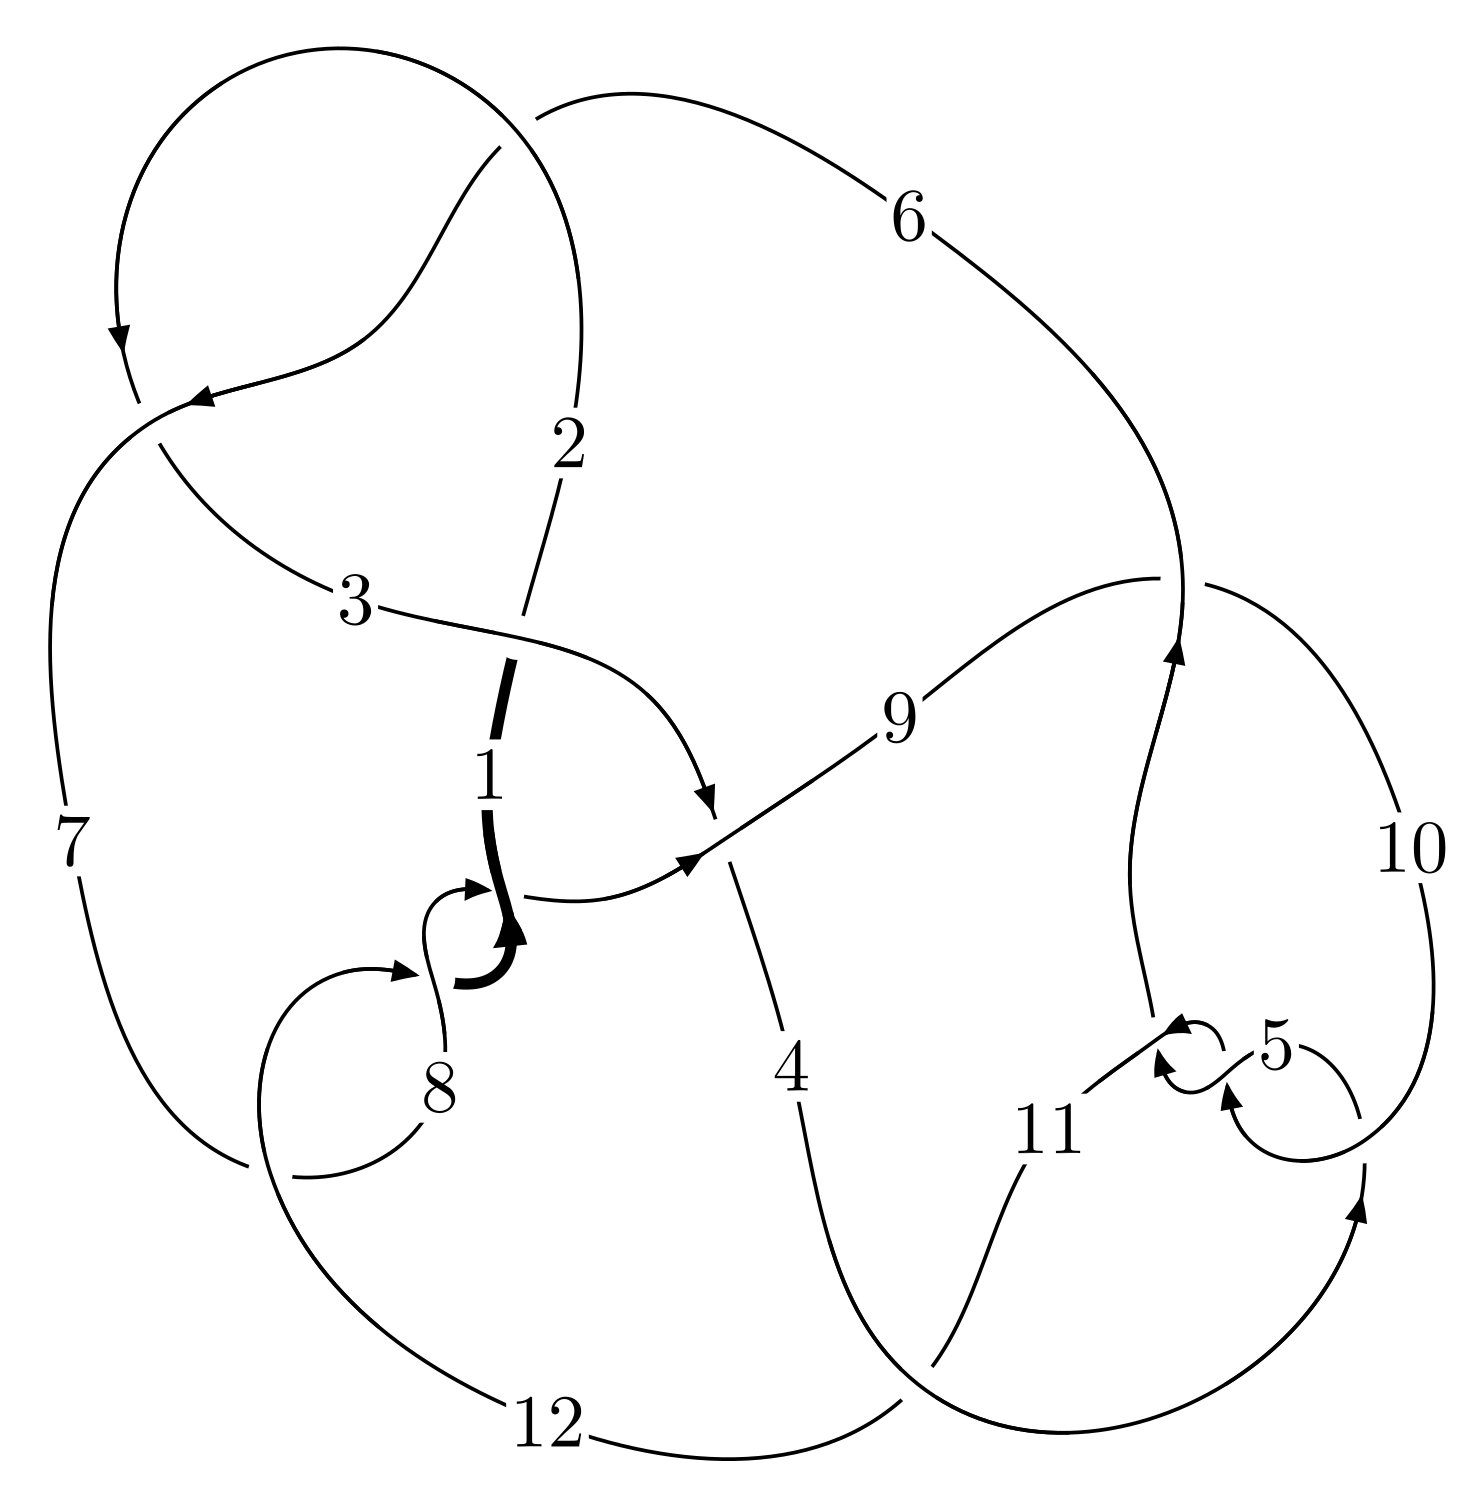
\includegraphics[width=112pt]{../../../GIT/diagram.site/Diagrams/png/1379_12a_0578.png}\\
\ \ \ A knot diagram\footnotemark}&
\allowdisplaybreaks
\textbf{Linearized knot diagam} \\
\cline{2-2}
 &
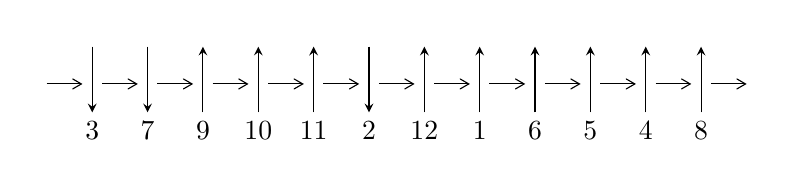
\begin{tikzpicture}[x=20pt, y=17pt]
	% nodes
	\node (C0) at (0, 0) {};
	\node (C1) at (1, 0) {};
	\node (C1U) at (1, +1) {};
	\node (C1D) at (1, -1) {3};

	\node (C2) at (2, 0) {};
	\node (C2U) at (2, +1) {};
	\node (C2D) at (2, -1) {7};

	\node (C3) at (3, 0) {};
	\node (C3U) at (3, +1) {};
	\node (C3D) at (3, -1) {9};

	\node (C4) at (4, 0) {};
	\node (C4U) at (4, +1) {};
	\node (C4D) at (4, -1) {10};

	\node (C5) at (5, 0) {};
	\node (C5U) at (5, +1) {};
	\node (C5D) at (5, -1) {11};

	\node (C6) at (6, 0) {};
	\node (C6U) at (6, +1) {};
	\node (C6D) at (6, -1) {2};

	\node (C7) at (7, 0) {};
	\node (C7U) at (7, +1) {};
	\node (C7D) at (7, -1) {12};

	\node (C8) at (8, 0) {};
	\node (C8U) at (8, +1) {};
	\node (C8D) at (8, -1) {1};

	\node (C9) at (9, 0) {};
	\node (C9U) at (9, +1) {};
	\node (C9D) at (9, -1) {6};

	\node (C10) at (10, 0) {};
	\node (C10U) at (10, +1) {};
	\node (C10D) at (10, -1) {5};

	\node (C11) at (11, 0) {};
	\node (C11U) at (11, +1) {};
	\node (C11D) at (11, -1) {4};

	\node (C12) at (12, 0) {};
	\node (C12U) at (12, +1) {};
	\node (C12D) at (12, -1) {8};
	\node (C13) at (13, 0) {};

	% arrows
	\draw[->,>={angle 60}]
	(C0) edge (C1) (C1) edge (C2) (C2) edge (C3) (C3) edge (C4) (C4) edge (C5) (C5) edge (C6) (C6) edge (C7) (C7) edge (C8) (C8) edge (C9) (C9) edge (C10) (C10) edge (C11) (C11) edge (C12) (C12) edge (C13) ;	\draw[->,>=stealth]
	(C1U) edge (C1D) (C2U) edge (C2D) (C3D) edge (C3U) (C4D) edge (C4U) (C5D) edge (C5U) (C6U) edge (C6D) (C7D) edge (C7U) (C8D) edge (C8U) (C9D) edge (C9U) (C10D) edge (C10U) (C11D) edge (C11U) (C12D) edge (C12U) ;
	\end{tikzpicture} \\
\hhline{~~} \\& 
\textbf{Solving Sequence} \\ \cline{2-2} 
 &
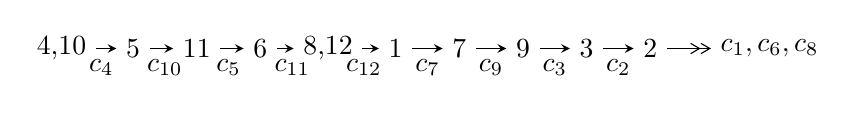
\begin{tikzpicture}[x=23pt, y=7pt]
	% node
	\node (A0) at (-1/8, 0) {4,10};
	\node (A1) at (1, 0) {5};
	\node (A2) at (2, 0) {11};
	\node (A3) at (3, 0) {6};
	\node (A4) at (65/16, 0) {8,12};
	\node (A5) at (41/8, 0) {1};
	\node (A6) at (49/8, 0) {7};
	\node (A7) at (57/8, 0) {9};
	\node (A8) at (65/8, 0) {3};
	\node (A9) at (73/8, 0) {2};
	\node (C1) at (1/2, -1) {$c_{4}$};
	\node (C2) at (3/2, -1) {$c_{10}$};
	\node (C3) at (5/2, -1) {$c_{5}$};
	\node (C4) at (7/2, -1) {$c_{11}$};
	\node (C5) at (37/8, -1) {$c_{12}$};
	\node (C6) at (45/8, -1) {$c_{7}$};
	\node (C7) at (53/8, -1) {$c_{9}$};
	\node (C8) at (61/8, -1) {$c_{3}$};
	\node (C9) at (69/8, -1) {$c_{2}$};
	\node (A10) at (11, 0) {$c_{1},c_{6},c_{8}$};

	% edge
	\draw[->,>=stealth]	
	(A0) edge (A1) (A1) edge (A2) (A2) edge (A3) (A3) edge (A4) (A4) edge (A5) (A5) edge (A6) (A6) edge (A7) (A7) edge (A8) (A8) edge (A9) ;
	\draw[->>,>={angle 60}]	
	(A9) edge (A10);
\end{tikzpicture} \\ 

\end{tabular} \\

\footnotetext{
The image of knot diagram is generated by the software ``\textbf{Draw programme}" developed by Andrew Bartholomew(\url{http://www.layer8.co.uk/maths/draw/index.htm\#Running-draw}), where we modified some parts for our purpose(\url{https://github.com/CATsTAILs/LinksPainter}).
}\phantom \\ \newline 
\centering \textbf{Ideals for irreducible components\footnotemark of $X_{\text{par}}$} 
 
\begin{align*}
I^u_{1}&=\langle 
- u^{58}+24 u^{56}+\cdots+4 b-4 u,\;u^{56}-23 u^{54}+\cdots+4 a+2,\;u^{61}-2 u^{60}+\cdots+2 u+2\rangle \\
I^u_{2}&=\langle 
474 u^7 a^2+726 u^7 a+\cdots+845 a+670,\;2 u^7 a^2+4 u^7 a+\cdots+4 a+2,\;u^8+u^7-3 u^6-2 u^5+3 u^4+2 u-1\rangle \\
I^u_{3}&=\langle 
b-1,\;2 u^3-3 u^2+3 a-3 u+3,\;u^4-3 u^2+3\rangle \\
I^u_{4}&=\langle 
b+1,\;- u^2+a+u+1,\;u^4- u^2-1\rangle \\
\\
I^v_{1}&=\langle 
a,\;b-1,\;v-1\rangle \\
\end{align*}
\raggedright * 5 irreducible components of $\dim_{\mathbb{C}}=0$, with total 94 representations.\\
\footnotetext{All coefficients of polynomials are rational numbers. But the coefficients are sometimes approximated in decimal forms when there is not enough margin.}
\newpage
\renewcommand{\arraystretch}{1}
\centering \section*{I. $I^u_{1}= \langle - u^{58}+24 u^{56}+\cdots+4 b-4 u,\;u^{56}-23 u^{54}+\cdots+4 a+2,\;u^{61}-2 u^{60}+\cdots+2 u+2 \rangle$}
\flushleft \textbf{(i) Arc colorings}\\
\begin{tabular}{m{7pt} m{180pt} m{7pt} m{180pt} }
\flushright $a_{4}=$&$\begin{pmatrix}1\\0\end{pmatrix}$ \\
\flushright $a_{10}=$&$\begin{pmatrix}0\\u\end{pmatrix}$ \\
\flushright $a_{5}=$&$\begin{pmatrix}1\\- u^2\end{pmatrix}$ \\
\flushright $a_{11}=$&$\begin{pmatrix}u\\- u^3+u\end{pmatrix}$ \\
\flushright $a_{6}=$&$\begin{pmatrix}- u^2+1\\u^4-2 u^2\end{pmatrix}$ \\
\flushright $a_{8}=$&$\begin{pmatrix}-\frac{1}{4} u^{56}+\frac{23}{4} u^{54}+\cdots-\frac{3}{2} u-\frac{1}{2}\\\frac{1}{4} u^{58}-6 u^{56}+\cdots+u^2+u\end{pmatrix}$ \\
\flushright $a_{12}=$&$\begin{pmatrix}- u^3+2 u\\- u^3+u\end{pmatrix}$ \\
\flushright $a_{1}=$&$\begin{pmatrix}-\frac{1}{4} u^{54}+\frac{23}{4} u^{52}+\cdots+\frac{5}{2} u+\frac{1}{2}\\-\frac{1}{4} u^{54}+\frac{11}{2} u^{52}+\cdots-4 u^3+u\end{pmatrix}$ \\
\flushright $a_{7}=$&$\begin{pmatrix}-\frac{1}{2} u^{60}+u^{59}+\cdots-\frac{3}{2} u-\frac{1}{2}\\- u^{60}+u^{59}+\cdots+\frac{5}{2} u+1\end{pmatrix}$ \\
\flushright $a_{9}=$&$\begin{pmatrix}- u^5+2 u^3- u\\u^7-3 u^5+2 u^3+u\end{pmatrix}$ \\
\flushright $a_{3}=$&$\begin{pmatrix}- u^{12}+5 u^{10}-9 u^8+6 u^6- u^2+1\\u^{14}-6 u^{12}+13 u^{10}-10 u^8-2 u^6+4 u^4+u^2\end{pmatrix}$ \\
\flushright $a_{2}=$&$\begin{pmatrix}-\frac{1}{4} u^{57}+6 u^{55}+\cdots+u+1\\-\frac{1}{4} u^{57}+\frac{23}{4} u^{55}+\cdots+\frac{1}{2} u^2+\frac{1}{2} u\end{pmatrix}$\\&\end{tabular}
\flushleft \textbf{(ii) Obstruction class $= -1$}\\~\\
\flushleft \textbf{(iii) Cusp Shapes $= -2 u^{60}+50 u^{58}+\cdots+20 u+12$}\\~\\
\newpage\renewcommand{\arraystretch}{1}
\flushleft \textbf{(iv) u-Polynomials at the component}\newline \\
\begin{tabular}{m{50pt}|m{274pt}}
Crossings & \hspace{64pt}u-Polynomials at each crossing \\
\hline $$\begin{aligned}c_{1}\end{aligned}$$&$\begin{aligned}
&u^{61}+24 u^{60}+\cdots+3579 u+49
\end{aligned}$\\
\hline $$\begin{aligned}c_{2},c_{6}\end{aligned}$$&$\begin{aligned}
&u^{61}-2 u^{60}+\cdots+31 u+7
\end{aligned}$\\
\hline $$\begin{aligned}c_{3}\end{aligned}$$&$\begin{aligned}
&u^{61}+2 u^{60}+\cdots-9398 u+5482
\end{aligned}$\\
\hline $$\begin{aligned}c_{4},c_{5},c_{10}\end{aligned}$$&$\begin{aligned}
&u^{61}-2 u^{60}+\cdots+2 u+2
\end{aligned}$\\
\hline $$\begin{aligned}c_{7},c_{8},c_{12}\end{aligned}$$&$\begin{aligned}
&u^{61}+2 u^{60}+\cdots-69 u+7
\end{aligned}$\\
\hline $$\begin{aligned}c_{9},c_{11}\end{aligned}$$&$\begin{aligned}
&u^{61}+6 u^{60}+\cdots+736 u+128
\end{aligned}$\\
\hline
\end{tabular}\\~\\
\newpage\renewcommand{\arraystretch}{1}
\flushleft \textbf{(v) Riley Polynomials at the component}\newline \\
\begin{tabular}{m{50pt}|m{274pt}}
Crossings & \hspace{64pt}Riley Polynomials at each crossing \\
\hline $$\begin{aligned}c_{1}\end{aligned}$$&$\begin{aligned}
&y^{61}+36 y^{60}+\cdots+7535175 y-2401
\end{aligned}$\\
\hline $$\begin{aligned}c_{2},c_{6}\end{aligned}$$&$\begin{aligned}
&y^{61}-24 y^{60}+\cdots+3579 y-49
\end{aligned}$\\
\hline $$\begin{aligned}c_{3}\end{aligned}$$&$\begin{aligned}
&y^{61}-10 y^{60}+\cdots-675769720 y-30052324
\end{aligned}$\\
\hline $$\begin{aligned}c_{4},c_{5},c_{10}\end{aligned}$$&$\begin{aligned}
&y^{61}-50 y^{60}+\cdots+8 y-4
\end{aligned}$\\
\hline $$\begin{aligned}c_{7},c_{8},c_{12}\end{aligned}$$&$\begin{aligned}
&y^{61}-64 y^{60}+\cdots+4075 y-49
\end{aligned}$\\
\hline $$\begin{aligned}c_{9},c_{11}\end{aligned}$$&$\begin{aligned}
&y^{61}+38 y^{60}+\cdots+115712 y-16384
\end{aligned}$\\
\hline
\end{tabular}\\~\\
\newpage\flushleft \textbf{(vi) Complex Volumes and Cusp Shapes}
$$\begin{array}{c|c|c}  
\text{Solutions to }I^u_{1}& \I (\text{vol} + \sqrt{-1}CS) & \text{Cusp shape}\\
 \hline 
\begin{aligned}
u &= -1.045080 + 0.313421 I \\
a &= \phantom{-}1.89893 - 0.49988 I \\
b &= \phantom{-}1.88740 + 0.56009 I\end{aligned}
 & \phantom{-}6.47668 + 1.81251 I & \phantom{-0.000000 } 0 \\ \hline\begin{aligned}
u &= -1.045080 - 0.313421 I \\
a &= \phantom{-}1.89893 + 0.49988 I \\
b &= \phantom{-}1.88740 - 0.56009 I\end{aligned}
 & \phantom{-}6.47668 - 1.81251 I & \phantom{-0.000000 } 0 \\ \hline\begin{aligned}
u &= \phantom{-}1.082430 + 0.367312 I \\
a &= -1.87282 - 0.76181 I \\
b &= -2.11893 + 0.51520 I\end{aligned}
 & \phantom{-}4.29961 - 7.38307 I & \phantom{-0.000000 } 0 \\ \hline\begin{aligned}
u &= \phantom{-}1.082430 - 0.367312 I \\
a &= -1.87282 + 0.76181 I \\
b &= -2.11893 - 0.51520 I\end{aligned}
 & \phantom{-}4.29961 + 7.38307 I & \phantom{-0.000000 } 0 \\ \hline\begin{aligned}
u &= \phantom{-}0.026391 + 0.841561 I \\
a &= \phantom{-}0.017329 - 0.723163 I \\
b &= \phantom{-}0.0358248 + 0.1097390 I\end{aligned}
 & -2.59755 - 1.90534 I & \phantom{-}5.48183 + 3.73036 I \\ \hline\begin{aligned}
u &= \phantom{-}0.026391 - 0.841561 I \\
a &= \phantom{-}0.017329 + 0.723163 I \\
b &= \phantom{-}0.0358248 - 0.1097390 I\end{aligned}
 & -2.59755 + 1.90534 I & \phantom{-}5.48183 - 3.73036 I \\ \hline\begin{aligned}
u &= -1.116950 + 0.320702 I \\
a &= -0.591762 + 0.486353 I \\
b &= -0.901647 - 0.672603 I\end{aligned}
 & -1.11946 + 3.33466 I & \phantom{-0.000000 } 0 \\ \hline\begin{aligned}
u &= -1.116950 - 0.320702 I \\
a &= -0.591762 - 0.486353 I \\
b &= -0.901647 + 0.672603 I\end{aligned}
 & -1.11946 - 3.33466 I & \phantom{-0.000000 } 0 \\ \hline\begin{aligned}
u &= \phantom{-}0.148036 + 0.815189 I \\
a &= \phantom{-}3.32481 + 2.12115 I \\
b &= \phantom{-}2.47279 + 0.61911 I\end{aligned}
 & \phantom{-}1.44711 + 11.68910 I & \phantom{-}5.41407 - 7.67902 I \\ \hline\begin{aligned}
u &= \phantom{-}0.148036 - 0.815189 I \\
a &= \phantom{-}3.32481 - 2.12115 I \\
b &= \phantom{-}2.47279 - 0.61911 I\end{aligned}
 & \phantom{-}1.44711 - 11.68910 I & \phantom{-}5.41407 + 7.67902 I\\
 \hline 
 \end{array}$$\newpage$$\begin{array}{c|c|c}  
\text{Solutions to }I^u_{1}& \I (\text{vol} + \sqrt{-1}CS) & \text{Cusp shape}\\
 \hline 
\begin{aligned}
u &= -0.159456 + 0.787209 I \\
a &= -3.07363 + 2.55815 I \\
b &= -2.30891 + 0.83730 I\end{aligned}
 & \phantom{-}3.77656 - 5.89886 I & \phantom{-}8.15888 + 3.94613 I \\ \hline\begin{aligned}
u &= -0.159456 - 0.787209 I \\
a &= -3.07363 - 2.55815 I \\
b &= -2.30891 - 0.83730 I\end{aligned}
 & \phantom{-}3.77656 + 5.89886 I & \phantom{-}8.15888 - 3.94613 I \\ \hline\begin{aligned}
u &= -0.128661 + 0.790668 I \\
a &= \phantom{-}1.20590 - 0.92529 I \\
b &= \phantom{-}1.199370 - 0.497535 I\end{aligned}
 & -4.10929 - 7.41360 I & \phantom{-}1.61547 + 7.26505 I \\ \hline\begin{aligned}
u &= -0.128661 - 0.790668 I \\
a &= \phantom{-}1.20590 + 0.92529 I \\
b &= \phantom{-}1.199370 + 0.497535 I\end{aligned}
 & -4.10929 + 7.41360 I & \phantom{-}1.61547 - 7.26505 I \\ \hline\begin{aligned}
u &= -0.050353 + 0.793051 I \\
a &= \phantom{-}1.03212 - 1.57158 I \\
b &= \phantom{-}0.890863 - 0.963022 I\end{aligned}
 & -6.44106 - 0.24388 I & -3.18042 + 0.12157 I \\ \hline\begin{aligned}
u &= -0.050353 - 0.793051 I \\
a &= \phantom{-}1.03212 + 1.57158 I \\
b &= \phantom{-}0.890863 + 0.963022 I\end{aligned}
 & -6.44106 + 0.24388 I & -3.18042 - 0.12157 I \\ \hline\begin{aligned}
u &= -0.687219 + 0.308158 I \\
a &= \phantom{-}1.43674 - 0.19679 I \\
b &= \phantom{-}1.78452 + 0.21827 I\end{aligned}
 & \phantom{-}7.10517 - 1.78344 I & \phantom{-}12.35005 + 2.03995 I \\ \hline\begin{aligned}
u &= -0.687219 - 0.308158 I \\
a &= \phantom{-}1.43674 + 0.19679 I \\
b &= \phantom{-}1.78452 - 0.21827 I\end{aligned}
 & \phantom{-}7.10517 + 1.78344 I & \phantom{-}12.35005 - 2.03995 I \\ \hline\begin{aligned}
u &= \phantom{-}1.25692\phantom{ +0.000000I} \\
a &= -0.481060\phantom{ +0.000000I} \\
b &= \phantom{-}0.855799\phantom{ +0.000000I}\end{aligned}
 & \phantom{-}2.32742\phantom{ +0.000000I} & \phantom{-0.000000 } 0 \\ \hline\begin{aligned}
u &= -1.217190 + 0.340958 I \\
a &= -1.011960 + 0.019839 I \\
b &= -0.688579 - 1.089540 I\end{aligned}
 & -2.85750 - 3.85140 I & \phantom{-0.000000 } 0\\
 \hline 
 \end{array}$$\newpage$$\begin{array}{c|c|c}  
\text{Solutions to }I^u_{1}& \I (\text{vol} + \sqrt{-1}CS) & \text{Cusp shape}\\
 \hline 
\begin{aligned}
u &= -1.217190 - 0.340958 I \\
a &= -1.011960 - 0.019839 I \\
b &= -0.688579 + 1.089540 I\end{aligned}
 & -2.85750 + 3.85140 I & \phantom{-0.000000 } 0 \\ \hline\begin{aligned}
u &= \phantom{-}0.611451 + 0.390031 I \\
a &= -1.342980 - 0.209011 I \\
b &= -1.75805 + 0.23081 I\end{aligned}
 & \phantom{-}5.48935 + 7.39656 I & \phantom{-}9.73203 - 7.29176 I \\ \hline\begin{aligned}
u &= \phantom{-}0.611451 - 0.390031 I \\
a &= -1.342980 + 0.209011 I \\
b &= -1.75805 - 0.23081 I\end{aligned}
 & \phantom{-}5.48935 - 7.39656 I & \phantom{-}9.73203 + 7.29176 I \\ \hline\begin{aligned}
u &= -1.28941\phantom{ +0.000000I} \\
a &= \phantom{-}1.15132\phantom{ +0.000000I} \\
b &= -0.131178\phantom{ +0.000000I}\end{aligned}
 & \phantom{-}5.56027\phantom{ +0.000000I} & \phantom{-0.000000 } 0 \\ \hline\begin{aligned}
u &= -0.235942 + 0.661253 I \\
a &= -1.48007 + 2.97320 I \\
b &= -1.39466 + 0.87587 I\end{aligned}
 & \phantom{-}5.54702 - 1.76287 I & \phantom{-}9.26008 + 3.99131 I \\ \hline\begin{aligned}
u &= -0.235942 - 0.661253 I \\
a &= -1.48007 - 2.97320 I \\
b &= -1.39466 - 0.87587 I\end{aligned}
 & \phantom{-}5.54702 + 1.76287 I & \phantom{-}9.26008 - 3.99131 I \\ \hline\begin{aligned}
u &= \phantom{-}1.238810 + 0.387315 I \\
a &= \phantom{-}0.113664 - 0.741618 I \\
b &= \phantom{-}0.115647 + 0.168942 I\end{aligned}
 & \phantom{-}1.14891 + 6.31724 I & \phantom{-0.000000 } 0 \\ \hline\begin{aligned}
u &= \phantom{-}1.238810 - 0.387315 I \\
a &= \phantom{-}0.113664 + 0.741618 I \\
b &= \phantom{-}0.115647 - 0.168942 I\end{aligned}
 & \phantom{-}1.14891 - 6.31724 I & \phantom{-0.000000 } 0 \\ \hline\begin{aligned}
u &= -1.280270 + 0.275839 I \\
a &= -0.249437 - 0.922926 I \\
b &= \phantom{-}0.613860 + 0.196052 I\end{aligned}
 & \phantom{-}2.59552 - 4.85268 I & \phantom{-0.000000 } 0 \\ \hline\begin{aligned}
u &= -1.280270 - 0.275839 I \\
a &= -0.249437 + 0.922926 I \\
b &= \phantom{-}0.613860 - 0.196052 I\end{aligned}
 & \phantom{-}2.59552 + 4.85268 I & \phantom{-0.000000 } 0\\
 \hline 
 \end{array}$$\newpage$$\begin{array}{c|c|c}  
\text{Solutions to }I^u_{1}& \I (\text{vol} + \sqrt{-1}CS) & \text{Cusp shape}\\
 \hline 
\begin{aligned}
u &= \phantom{-}0.302742 + 0.600452 I \\
a &= \phantom{-}0.95957 + 2.68395 I \\
b &= \phantom{-}1.173020 + 0.631568 I\end{aligned}
 & \phantom{-}4.47511 - 3.82165 I & \phantom{-}8.02527 + 1.02116 I \\ \hline\begin{aligned}
u &= \phantom{-}0.302742 - 0.600452 I \\
a &= \phantom{-}0.95957 - 2.68395 I \\
b &= \phantom{-}1.173020 - 0.631568 I\end{aligned}
 & \phantom{-}4.47511 + 3.82165 I & \phantom{-}8.02527 - 1.02116 I \\ \hline\begin{aligned}
u &= -1.284030 + 0.381487 I \\
a &= -0.134033 - 0.700730 I \\
b &= -0.157554 + 0.062498 I\end{aligned}
 & \phantom{-}1.47922 - 2.48565 I & \phantom{-0.000000 } 0 \\ \hline\begin{aligned}
u &= -1.284030 - 0.381487 I \\
a &= -0.134033 + 0.700730 I \\
b &= -0.157554 - 0.062498 I\end{aligned}
 & \phantom{-}1.47922 + 2.48565 I & \phantom{-0.000000 } 0 \\ \hline\begin{aligned}
u &= \phantom{-}1.299870 + 0.344849 I \\
a &= \phantom{-}0.463664 - 1.207460 I \\
b &= -1.040970 - 0.847148 I\end{aligned}
 & -2.22544 + 4.34429 I & \phantom{-0.000000 } 0 \\ \hline\begin{aligned}
u &= \phantom{-}1.299870 - 0.344849 I \\
a &= \phantom{-}0.463664 + 1.207460 I \\
b &= -1.040970 + 0.847148 I\end{aligned}
 & -2.22544 - 4.34429 I & \phantom{-0.000000 } 0 \\ \hline\begin{aligned}
u &= \phantom{-}1.318970 + 0.274899 I \\
a &= \phantom{-}0.178307 - 0.453100 I \\
b &= \phantom{-}0.367203 - 0.307219 I\end{aligned}
 & \phantom{-}2.88323 + 1.86161 I & \phantom{-0.000000 } 0 \\ \hline\begin{aligned}
u &= \phantom{-}1.318970 - 0.274899 I \\
a &= \phantom{-}0.178307 + 0.453100 I \\
b &= \phantom{-}0.367203 + 0.307219 I\end{aligned}
 & \phantom{-}2.88323 - 1.86161 I & \phantom{-0.000000 } 0 \\ \hline\begin{aligned}
u &= -0.010977 + 0.647106 I \\
a &= -0.368429 - 0.667382 I \\
b &= -0.488496 + 0.022625 I\end{aligned}
 & -1.39623 + 1.46553 I & \phantom{-}4.80729 - 4.40781 I \\ \hline\begin{aligned}
u &= -0.010977 - 0.647106 I \\
a &= -0.368429 + 0.667382 I \\
b &= -0.488496 - 0.022625 I\end{aligned}
 & -1.39623 - 1.46553 I & \phantom{-}4.80729 + 4.40781 I\\
 \hline 
 \end{array}$$\newpage$$\begin{array}{c|c|c}  
\text{Solutions to }I^u_{1}& \I (\text{vol} + \sqrt{-1}CS) & \text{Cusp shape}\\
 \hline 
\begin{aligned}
u &= \phantom{-}1.383270 + 0.045423 I \\
a &= -0.445627 - 0.436211 I \\
b &= \phantom{-}0.630719 - 0.251341 I\end{aligned}
 & \phantom{-}5.65281 + 4.80409 I & \phantom{-0.000000 } 0 \\ \hline\begin{aligned}
u &= \phantom{-}1.383270 - 0.045423 I \\
a &= -0.445627 + 0.436211 I \\
b &= \phantom{-}0.630719 + 0.251341 I\end{aligned}
 & \phantom{-}5.65281 - 4.80409 I & \phantom{-0.000000 } 0 \\ \hline\begin{aligned}
u &= -1.368750 + 0.233531 I \\
a &= \phantom{-}1.10473 + 1.86272 I \\
b &= -1.17608 + 1.32230 I\end{aligned}
 & \phantom{-}9.69673 + 0.83184 I & \phantom{-0.000000 } 0 \\ \hline\begin{aligned}
u &= -1.368750 - 0.233531 I \\
a &= \phantom{-}1.10473 - 1.86272 I \\
b &= -1.17608 - 1.32230 I\end{aligned}
 & \phantom{-}9.69673 - 0.83184 I & \phantom{-0.000000 } 0 \\ \hline\begin{aligned}
u &= \phantom{-}1.346800 + 0.339601 I \\
a &= \phantom{-}0.168072 - 1.073780 I \\
b &= -1.370380 - 0.345312 I\end{aligned}
 & \phantom{-}0.53517 + 11.49560 I & \phantom{-0.000000 } 0 \\ \hline\begin{aligned}
u &= \phantom{-}1.346800 - 0.339601 I \\
a &= \phantom{-}0.168072 + 1.073780 I \\
b &= -1.370380 + 0.345312 I\end{aligned}
 & \phantom{-}0.53517 - 11.49560 I & \phantom{-0.000000 } 0 \\ \hline\begin{aligned}
u &= \phantom{-}1.368020 + 0.269439 I \\
a &= -0.92620 + 2.29059 I \\
b &= \phantom{-}1.61066 + 1.41688 I\end{aligned}
 & \phantom{-}10.58940 + 5.14714 I & \phantom{-0.000000 } 0 \\ \hline\begin{aligned}
u &= \phantom{-}1.368020 - 0.269439 I \\
a &= -0.92620 - 2.29059 I \\
b &= \phantom{-}1.61066 - 1.41688 I\end{aligned}
 & \phantom{-}10.58940 - 5.14714 I & \phantom{-0.000000 } 0 \\ \hline\begin{aligned}
u &= -0.536071 + 0.277726 I \\
a &= \phantom{-}0.182357 - 0.605325 I \\
b &= -0.358021 + 0.249835 I\end{aligned}
 & -0.27372 - 3.92540 I & \phantom{-}6.34246 + 7.90863 I \\ \hline\begin{aligned}
u &= -0.536071 - 0.277726 I \\
a &= \phantom{-}0.182357 + 0.605325 I \\
b &= -0.358021 - 0.249835 I\end{aligned}
 & -0.27372 + 3.92540 I & \phantom{-}6.34246 - 7.90863 I\\
 \hline 
 \end{array}$$\newpage$$\begin{array}{c|c|c}  
\text{Solutions to }I^u_{1}& \I (\text{vol} + \sqrt{-1}CS) & \text{Cusp shape}\\
 \hline 
\begin{aligned}
u &= \phantom{-}1.361620 + 0.334725 I \\
a &= \phantom{-}0.07582 + 2.89140 I \\
b &= \phantom{-}2.60850 + 0.92122 I\end{aligned}
 & \phantom{-}8.57491 + 9.95414 I & \phantom{-0.000000 } 0 \\ \hline\begin{aligned}
u &= \phantom{-}1.361620 - 0.334725 I \\
a &= \phantom{-}0.07582 - 2.89140 I \\
b &= \phantom{-}2.60850 - 0.92122 I\end{aligned}
 & \phantom{-}8.57491 - 9.95414 I & \phantom{-0.000000 } 0 \\ \hline\begin{aligned}
u &= -1.359900 + 0.350372 I \\
a &= -0.40622 + 2.83427 I \\
b &= -2.72449 + 0.62392 I\end{aligned}
 & \phantom{-}6.2004 - 15.8925 I & \phantom{-0.000000 } 0 \\ \hline\begin{aligned}
u &= -1.359900 - 0.350372 I \\
a &= -0.40622 - 2.83427 I \\
b &= -2.72449 - 0.62392 I\end{aligned}
 & \phantom{-}6.2004 + 15.8925 I & \phantom{-0.000000 } 0 \\ \hline\begin{aligned}
u &= \phantom{-}1.41422 + 0.03842 I \\
a &= \phantom{-}1.006490 - 0.306439 I \\
b &= -2.60422 + 0.34117 I\end{aligned}
 & \phantom{-}13.60740 + 2.58481 I & \phantom{-0.000000 } 0 \\ \hline\begin{aligned}
u &= \phantom{-}1.41422 - 0.03842 I \\
a &= \phantom{-}1.006490 + 0.306439 I \\
b &= -2.60422 - 0.34117 I\end{aligned}
 & \phantom{-}13.60740 - 2.58481 I & \phantom{-0.000000 } 0 \\ \hline\begin{aligned}
u &= -1.41341 + 0.06611 I \\
a &= -0.898179 - 0.480612 I \\
b &= \phantom{-}2.43333 + 0.51052 I\end{aligned}
 & \phantom{-}11.8693 - 8.6563 I & \phantom{-0.000000 } 0 \\ \hline\begin{aligned}
u &= -1.41341 - 0.06611 I \\
a &= -0.898179 + 0.480612 I \\
b &= \phantom{-}2.43333 - 0.51052 I\end{aligned}
 & \phantom{-}11.8693 + 8.6563 I & \phantom{-0.000000 } 0 \\ \hline\begin{aligned}
u &= -0.170322 + 0.434793 I \\
a &= -0.067068 - 0.388822 I \\
b &= -0.294850 + 0.289305 I\end{aligned}
 & -1.34960 + 1.22997 I & \phantom{-}1.31252 - 1.31517 I \\ \hline\begin{aligned}
u &= -0.170322 - 0.434793 I \\
a &= -0.067068 + 0.388822 I \\
b &= -0.294850 - 0.289305 I\end{aligned}
 & -1.34960 - 1.22997 I & \phantom{-}1.31252 + 1.31517 I\\
 \hline 
 \end{array}$$\newpage$$\begin{array}{c|c|c}  
\text{Solutions to }I^u_{1}& \I (\text{vol} + \sqrt{-1}CS) & \text{Cusp shape}\\
 \hline 
\begin{aligned}
u &= \phantom{-}0.356420\phantom{ +0.000000I} \\
a &= -1.27045\phantom{ +0.000000I} \\
b &= \phantom{-}0.399618\phantom{ +0.000000I}\end{aligned}
 & \phantom{-}0.765127\phantom{ +0.000000I} & \phantom{-}14.4300\phantom{ +0.000000I}\\
 \hline 
 \end{array}$$\newpage\newpage\renewcommand{\arraystretch}{1}
\centering \section*{II. $I^u_{2}= \langle 474 u^7 a^2+726 u^7 a+\cdots+845 a+670,\;2 u^7 a^2+4 u^7 a+\cdots+4 a+2,\;u^8+u^7-3 u^6-2 u^5+3 u^4+2 u-1 \rangle$}
\flushleft \textbf{(i) Arc colorings}\\
\begin{tabular}{m{7pt} m{180pt} m{7pt} m{180pt} }
\flushright $a_{4}=$&$\begin{pmatrix}1\\0\end{pmatrix}$ \\
\flushright $a_{10}=$&$\begin{pmatrix}0\\u\end{pmatrix}$ \\
\flushright $a_{5}=$&$\begin{pmatrix}1\\- u^2\end{pmatrix}$ \\
\flushright $a_{11}=$&$\begin{pmatrix}u\\- u^3+u\end{pmatrix}$ \\
\flushright $a_{6}=$&$\begin{pmatrix}- u^2+1\\u^4-2 u^2\end{pmatrix}$ \\
\flushright $a_{8}=$&$\begin{pmatrix}a\\-1.15892 a^{2} u^{7}-1.77506 a u^{7}+\cdots-2.06601 a-1.63814\end{pmatrix}$ \\
\flushright $a_{12}=$&$\begin{pmatrix}- u^3+2 u\\- u^3+u\end{pmatrix}$ \\
\flushright $a_{1}=$&$\begin{pmatrix}-1.15892 a^{2} u^{7}-1.77506 a u^{7}+\cdots-3.06601 a-1.63814\\-0.205379 a^{2} u^{7}-1.12469 a u^{7}+\cdots-1.66993 a-1.80929\end{pmatrix}$ \\
\flushright $a_{7}=$&$\begin{pmatrix}0.256724 a^{2} u^{7}+0.405868 a u^{7}+\cdots+3.33741 a+1.26161\\-1.08802 a^{2} u^{7}-2.76773 a u^{7}+\cdots-0.144254 a-1.06112\end{pmatrix}$ \\
\flushright $a_{9}=$&$\begin{pmatrix}- u^5+2 u^3- u\\u^7-3 u^5+2 u^3+u\end{pmatrix}$ \\
\flushright $a_{3}=$&$\begin{pmatrix}- u^3+2 u\\- u^3+u\end{pmatrix}$ \\
\flushright $a_{2}=$&$\begin{pmatrix}-0.513447 a^{2} u^{7}-1.81174 a u^{7}+\cdots-2.67482 a-2.52323\\-0.398533 a^{2} u^{7}-0.420538 a u^{7}+\cdots-2.18093 a-2.41565\end{pmatrix}$\\&\end{tabular}
\flushleft \textbf{(ii) Obstruction class $= -1$}\\~\\
\flushleft \textbf{(iii) Cusp Shapes $= 4 u^6-12 u^4+4 u^3+8 u^2-8 u+14$}\\~\\
\newpage\renewcommand{\arraystretch}{1}
\flushleft \textbf{(iv) u-Polynomials at the component}\newline \\
\begin{tabular}{m{50pt}|m{274pt}}
Crossings & \hspace{64pt}u-Polynomials at each crossing \\
\hline $$\begin{aligned}c_{1}\end{aligned}$$&$\begin{aligned}
&u^{24}+16 u^{23}+\cdots+4 u+1
\end{aligned}$\\
\hline $$\begin{aligned}c_{2},c_{6},c_{7}\\c_{8},c_{12}\end{aligned}$$&$\begin{aligned}
&u^{24}-8 u^{22}+\cdots+2 u-1
\end{aligned}$\\
\hline $$\begin{aligned}c_{3}\end{aligned}$$&$\begin{aligned}
&(u^8- u^7- u^6+2 u^5+u^4-2 u^3+2 u-1)^3
\end{aligned}$\\
\hline $$\begin{aligned}c_{4},c_{5},c_{10}\end{aligned}$$&$\begin{aligned}
&(u^8+u^7-3 u^6-2 u^5+3 u^4+2 u-1)^3
\end{aligned}$\\
\hline $$\begin{aligned}c_{9},c_{11}\end{aligned}$$&$\begin{aligned}
&(u^8-3 u^7+7 u^6-10 u^5+11 u^4-10 u^3+6 u^2-4 u+1)^3
\end{aligned}$\\
\hline
\end{tabular}\\~\\
\newpage\renewcommand{\arraystretch}{1}
\flushleft \textbf{(v) Riley Polynomials at the component}\newline \\
\begin{tabular}{m{50pt}|m{274pt}}
Crossings & \hspace{64pt}Riley Polynomials at each crossing \\
\hline $$\begin{aligned}c_{1}\end{aligned}$$&$\begin{aligned}
&y^{24}-16 y^{23}+\cdots+12 y+1
\end{aligned}$\\
\hline $$\begin{aligned}c_{2},c_{6},c_{7}\\c_{8},c_{12}\end{aligned}$$&$\begin{aligned}
&y^{24}-16 y^{23}+\cdots-4 y+1
\end{aligned}$\\
\hline $$\begin{aligned}c_{3}\end{aligned}$$&$\begin{aligned}
&(y^8-3 y^7+7 y^6-10 y^5+11 y^4-10 y^3+6 y^2-4 y+1)^3
\end{aligned}$\\
\hline $$\begin{aligned}c_{4},c_{5},c_{10}\end{aligned}$$&$\begin{aligned}
&(y^8-7 y^7+19 y^6-22 y^5+3 y^4+14 y^3-6 y^2-4 y+1)^3
\end{aligned}$\\
\hline $$\begin{aligned}c_{9},c_{11}\end{aligned}$$&$\begin{aligned}
&(y^8+5 y^7+11 y^6+6 y^5-17 y^4-34 y^3-22 y^2-4 y+1)^3
\end{aligned}$\\
\hline
\end{tabular}\\~\\
\newpage\flushleft \textbf{(vi) Complex Volumes and Cusp Shapes}
$$\begin{array}{c|c|c}  
\text{Solutions to }I^u_{2}& \I (\text{vol} + \sqrt{-1}CS) & \text{Cusp shape}\\
 \hline 
\begin{aligned}
u &= \phantom{-}1.180120 + 0.268597 I \\
a &= \phantom{-}0.076281 - 0.895533 I \\
b &= -0.077043 + 0.520180 I\end{aligned}
 & \phantom{-}1.04066 + 1.13123 I & \phantom{-}7.41522 - 0.51079 I \\ \hline\begin{aligned}
u &= \phantom{-}1.180120 + 0.268597 I \\
a &= \phantom{-}0.459141 + 0.156574 I \\
b &= \phantom{-}0.701428 - 0.662460 I\end{aligned}
 & \phantom{-}1.04066 + 1.13123 I & \phantom{-}7.41522 - 0.51079 I \\ \hline\begin{aligned}
u &= \phantom{-}1.180120 + 0.268597 I \\
a &= -2.78777 - 0.16222 I \\
b &= -1.76612 + 1.60362 I\end{aligned}
 & \phantom{-}1.04066 + 1.13123 I & \phantom{-}7.41522 - 0.51079 I \\ \hline\begin{aligned}
u &= \phantom{-}1.180120 - 0.268597 I \\
a &= \phantom{-}0.076281 + 0.895533 I \\
b &= -0.077043 - 0.520180 I\end{aligned}
 & \phantom{-}1.04066 - 1.13123 I & \phantom{-}7.41522 + 0.51079 I \\ \hline\begin{aligned}
u &= \phantom{-}1.180120 - 0.268597 I \\
a &= \phantom{-}0.459141 - 0.156574 I \\
b &= \phantom{-}0.701428 + 0.662460 I\end{aligned}
 & \phantom{-}1.04066 - 1.13123 I & \phantom{-}7.41522 + 0.51079 I \\ \hline\begin{aligned}
u &= \phantom{-}1.180120 - 0.268597 I \\
a &= -2.78777 + 0.16222 I \\
b &= -1.76612 - 1.60362 I\end{aligned}
 & \phantom{-}1.04066 - 1.13123 I & \phantom{-}7.41522 + 0.51079 I \\ \hline\begin{aligned}
u &= \phantom{-}0.108090 + 0.747508 I \\
a &= \phantom{-}0.113638 - 0.691981 I \\
b &= \phantom{-}0.212333 + 0.099676 I\end{aligned}
 & -2.15941 + 2.57849 I & \phantom{-}4.27708 - 3.56796 I \\ \hline\begin{aligned}
u &= \phantom{-}0.108090 + 0.747508 I \\
a &= -0.963002 - 0.938902 I \\
b &= -0.991467 - 0.421518 I\end{aligned}
 & -2.15941 + 2.57849 I & \phantom{-}4.27708 - 3.56796 I \\ \hline\begin{aligned}
u &= \phantom{-}0.108090 + 0.747508 I \\
a &= \phantom{-}3.56457 + 3.92845 I \\
b &= \phantom{-}2.48961 + 1.65363 I\end{aligned}
 & -2.15941 + 2.57849 I & \phantom{-}4.27708 - 3.56796 I \\ \hline\begin{aligned}
u &= \phantom{-}0.108090 - 0.747508 I \\
a &= \phantom{-}0.113638 + 0.691981 I \\
b &= \phantom{-}0.212333 - 0.099676 I\end{aligned}
 & -2.15941 - 2.57849 I & \phantom{-}4.27708 + 3.56796 I\\
 \hline 
 \end{array}$$\newpage$$\begin{array}{c|c|c}  
\text{Solutions to }I^u_{2}& \I (\text{vol} + \sqrt{-1}CS) & \text{Cusp shape}\\
 \hline 
\begin{aligned}
u &= \phantom{-}0.108090 - 0.747508 I \\
a &= -0.963002 + 0.938902 I \\
b &= -0.991467 + 0.421518 I\end{aligned}
 & -2.15941 - 2.57849 I & \phantom{-}4.27708 + 3.56796 I \\ \hline\begin{aligned}
u &= \phantom{-}0.108090 - 0.747508 I \\
a &= \phantom{-}3.56457 - 3.92845 I \\
b &= \phantom{-}2.48961 - 1.65363 I\end{aligned}
 & -2.15941 - 2.57849 I & \phantom{-}4.27708 + 3.56796 I \\ \hline\begin{aligned}
u &= -1.37100\phantom{ +0.000000I} \\
a &= \phantom{-}0.636845 + 0.458999 I \\
b &= -0.572115 + 0.288256 I\end{aligned}
 & \phantom{-}6.50273\phantom{ +0.000000I} & \phantom{-}13.8640\phantom{ +0.000000I} \\ \hline\begin{aligned}
u &= -1.37100\phantom{ +0.000000I} \\
a &= \phantom{-}0.636845 - 0.458999 I \\
b &= -0.572115 - 0.288256 I\end{aligned}
 & \phantom{-}6.50273\phantom{ +0.000000I} & \phantom{-}13.8640\phantom{ +0.000000I} \\ \hline\begin{aligned}
u &= -1.37100\phantom{ +0.000000I} \\
a &= -1.57420\phantom{ +0.000000I} \\
b &= \phantom{-}3.34059\phantom{ +0.000000I}\end{aligned}
 & \phantom{-}6.50273\phantom{ +0.000000I} & \phantom{-}13.8640\phantom{ +0.000000I} \\ \hline\begin{aligned}
u &= -1.334530 + 0.318930 I \\
a &= -0.244708 - 1.025470 I \\
b &= \phantom{-}1.179160 - 0.265563 I\end{aligned}
 & \phantom{-}2.37968 - 6.44354 I & \phantom{-}9.42845 + 5.29417 I \\ \hline\begin{aligned}
u &= -1.334530 + 0.318930 I \\
a &= -0.156204 - 0.575525 I \\
b &= -0.287346 - 0.164227 I\end{aligned}
 & \phantom{-}2.37968 - 6.44354 I & \phantom{-}9.42845 + 5.29417 I \\ \hline\begin{aligned}
u &= -1.334530 + 0.318930 I \\
a &= \phantom{-}0.46011 + 3.64228 I \\
b &= -2.95543 + 1.74073 I\end{aligned}
 & \phantom{-}2.37968 - 6.44354 I & \phantom{-}9.42845 + 5.29417 I \\ \hline\begin{aligned}
u &= -1.334530 - 0.318930 I \\
a &= -0.244708 + 1.025470 I \\
b &= \phantom{-}1.179160 + 0.265563 I\end{aligned}
 & \phantom{-}2.37968 + 6.44354 I & \phantom{-}9.42845 - 5.29417 I \\ \hline\begin{aligned}
u &= -1.334530 - 0.318930 I \\
a &= -0.156204 + 0.575525 I \\
b &= -0.287346 + 0.164227 I\end{aligned}
 & \phantom{-}2.37968 + 6.44354 I & \phantom{-}9.42845 - 5.29417 I\\
 \hline 
 \end{array}$$\newpage$$\begin{array}{c|c|c}  
\text{Solutions to }I^u_{2}& \I (\text{vol} + \sqrt{-1}CS) & \text{Cusp shape}\\
 \hline 
\begin{aligned}
u &= -1.334530 - 0.318930 I \\
a &= \phantom{-}0.46011 - 3.64228 I \\
b &= -2.95543 - 1.74073 I\end{aligned}
 & \phantom{-}2.37968 + 6.44354 I & \phantom{-}9.42845 - 5.29417 I \\ \hline\begin{aligned}
u &= \phantom{-}0.463640\phantom{ +0.000000I} \\
a &= -0.636726 + 0.745558 I \\
b &= \phantom{-}0.458330 - 0.091081 I\end{aligned}
 & \phantom{-}0.845036\phantom{ +0.000000I} & \phantom{-}11.8940\phantom{ +0.000000I} \\ \hline\begin{aligned}
u &= \phantom{-}0.463640\phantom{ +0.000000I} \\
a &= -0.636726 - 0.745558 I \\
b &= \phantom{-}0.458330 + 0.091081 I\end{aligned}
 & \phantom{-}0.845036\phantom{ +0.000000I} & \phantom{-}11.8940\phantom{ +0.000000I} \\ \hline\begin{aligned}
u &= \phantom{-}0.463640\phantom{ +0.000000I} \\
a &= -1.47016\phantom{ +0.000000I} \\
b &= -2.12327\phantom{ +0.000000I}\end{aligned}
 & \phantom{-}0.845036\phantom{ +0.000000I} & \phantom{-}11.8940\phantom{ +0.000000I}\\
 \hline 
 \end{array}$$\newpage\newpage\renewcommand{\arraystretch}{1}
\centering \section*{III. $I^u_{3}= \langle b-1,\;2 u^3-3 u^2+3 a-3 u+3,\;u^4-3 u^2+3 \rangle$}
\flushleft \textbf{(i) Arc colorings}\\
\begin{tabular}{m{7pt} m{180pt} m{7pt} m{180pt} }
\flushright $a_{4}=$&$\begin{pmatrix}1\\0\end{pmatrix}$ \\
\flushright $a_{10}=$&$\begin{pmatrix}0\\u\end{pmatrix}$ \\
\flushright $a_{5}=$&$\begin{pmatrix}1\\- u^2\end{pmatrix}$ \\
\flushright $a_{11}=$&$\begin{pmatrix}u\\- u^3+u\end{pmatrix}$ \\
\flushright $a_{6}=$&$\begin{pmatrix}- u^2+1\\u^2-3\end{pmatrix}$ \\
\flushright $a_{8}=$&$\begin{pmatrix}-\frac{2}{3} u^3+u^2+u-1\\1\end{pmatrix}$ \\
\flushright $a_{12}=$&$\begin{pmatrix}- u^3+2 u\\- u^3+u\end{pmatrix}$ \\
\flushright $a_{1}=$&$\begin{pmatrix}-\frac{1}{3} u^3- u^2+u+1\\- u^3+u-1\end{pmatrix}$ \\
\flushright $a_{7}=$&$\begin{pmatrix}\frac{1}{3} u^3+u^2- u-1\\u^3- u+1\end{pmatrix}$ \\
\flushright $a_{9}=$&$\begin{pmatrix}- u^3+2 u\\- u^3+u\end{pmatrix}$ \\
\flushright $a_{3}=$&$\begin{pmatrix}- u^2+1\\u^2-3\end{pmatrix}$ \\
\flushright $a_{2}=$&$\begin{pmatrix}-\frac{1}{3} u^3-2 u^2+u+2\\- u^3+u^2+u-4\end{pmatrix}$\\&\end{tabular}
\flushleft \textbf{(ii) Obstruction class $= 1$}\\~\\
\flushleft \textbf{(iii) Cusp Shapes $= -4 u^2+12$}\\~\\
\newpage\renewcommand{\arraystretch}{1}
\flushleft \textbf{(iv) u-Polynomials at the component}\newline \\
\begin{tabular}{m{50pt}|m{274pt}}
Crossings & \hspace{64pt}u-Polynomials at each crossing \\
\hline $$\begin{aligned}c_{1},c_{2},c_{12}\end{aligned}$$&$\begin{aligned}
&(u-1)^4
\end{aligned}$\\
\hline $$\begin{aligned}c_{3},c_{9},c_{11}\end{aligned}$$&$\begin{aligned}
&u^4+3 u^2+3
\end{aligned}$\\
\hline $$\begin{aligned}c_{4},c_{5},c_{10}\end{aligned}$$&$\begin{aligned}
&u^4-3 u^2+3
\end{aligned}$\\
\hline $$\begin{aligned}c_{6},c_{7},c_{8}\end{aligned}$$&$\begin{aligned}
&(u+1)^4
\end{aligned}$\\
\hline
\end{tabular}\\~\\
\newpage\renewcommand{\arraystretch}{1}
\flushleft \textbf{(v) Riley Polynomials at the component}\newline \\
\begin{tabular}{m{50pt}|m{274pt}}
Crossings & \hspace{64pt}Riley Polynomials at each crossing \\
\hline $$\begin{aligned}c_{1},c_{2},c_{6}\\c_{7},c_{8},c_{12}\end{aligned}$$&$\begin{aligned}
&(y-1)^4
\end{aligned}$\\
\hline $$\begin{aligned}c_{3},c_{9},c_{11}\end{aligned}$$&$\begin{aligned}
&(y^2+3 y+3)^2
\end{aligned}$\\
\hline $$\begin{aligned}c_{4},c_{5},c_{10}\end{aligned}$$&$\begin{aligned}
&(y^2-3 y+3)^2
\end{aligned}$\\
\hline
\end{tabular}\\~\\
\newpage\flushleft \textbf{(vi) Complex Volumes and Cusp Shapes}
$$\begin{array}{c|c|c}  
\text{Solutions to }I^u_{3}& \I (\text{vol} + \sqrt{-1}CS) & \text{Cusp shape}\\
 \hline 
\begin{aligned}
u &= \phantom{-}1.271230 + 0.340625 I \\
a &= \phantom{-}0.696660 + 0.132080 I \\
b &= \phantom{-}1.00000\phantom{ +0.000000I}\end{aligned}
 & \phantom{-0.000000 -}4.05977 I & \phantom{-}6.00000 - 3.46410 I \\ \hline\begin{aligned}
u &= \phantom{-}1.271230 - 0.340625 I \\
a &= \phantom{-}0.696660 - 0.132080 I \\
b &= \phantom{-}1.00000\phantom{ +0.000000I}\end{aligned}
 & \phantom{-0.000000 } -4.05977 I & \phantom{-}6.00000 + 3.46410 I \\ \hline\begin{aligned}
u &= -1.271230 + 0.340625 I \\
a &= \phantom{-}0.30334 - 1.59997 I \\
b &= \phantom{-}1.00000\phantom{ +0.000000I}\end{aligned}
 & \phantom{-0.000000 } -4.05977 I & \phantom{-}6.00000 + 3.46410 I \\ \hline\begin{aligned}
u &= -1.271230 - 0.340625 I \\
a &= \phantom{-}0.30334 + 1.59997 I \\
b &= \phantom{-}1.00000\phantom{ +0.000000I}\end{aligned}
 & \phantom{-0.000000 -}4.05977 I & \phantom{-}6.00000 - 3.46410 I\\
 \hline 
 \end{array}$$\newpage\newpage\renewcommand{\arraystretch}{1}
\centering \section*{IV. $I^u_{4}= \langle b+1,\;- u^2+a+u+1,\;u^4- u^2-1 \rangle$}
\flushleft \textbf{(i) Arc colorings}\\
\begin{tabular}{m{7pt} m{180pt} m{7pt} m{180pt} }
\flushright $a_{4}=$&$\begin{pmatrix}1\\0\end{pmatrix}$ \\
\flushright $a_{10}=$&$\begin{pmatrix}0\\u\end{pmatrix}$ \\
\flushright $a_{5}=$&$\begin{pmatrix}1\\- u^2\end{pmatrix}$ \\
\flushright $a_{11}=$&$\begin{pmatrix}u\\- u^3+u\end{pmatrix}$ \\
\flushright $a_{6}=$&$\begin{pmatrix}- u^2+1\\- u^2+1\end{pmatrix}$ \\
\flushright $a_{8}=$&$\begin{pmatrix}u^2- u-1\\-1\end{pmatrix}$ \\
\flushright $a_{12}=$&$\begin{pmatrix}- u^3+2 u\\- u^3+u\end{pmatrix}$ \\
\flushright $a_{1}=$&$\begin{pmatrix}- u^3+u^2+u-1\\- u^3+u-1\end{pmatrix}$ \\
\flushright $a_{7}=$&$\begin{pmatrix}- u^3+u^2+u-1\\- u^3+u-1\end{pmatrix}$ \\
\flushright $a_{9}=$&$\begin{pmatrix}u^3-2 u\\u^3- u\end{pmatrix}$ \\
\flushright $a_{3}=$&$\begin{pmatrix}u^2-1\\u^2-1\end{pmatrix}$ \\
\flushright $a_{2}=$&$\begin{pmatrix}- u^3+2 u^2+u-2\\- u^3+u^2+u-2\end{pmatrix}$\\&\end{tabular}
\flushleft \textbf{(ii) Obstruction class $= 1$}\\~\\
\flushleft \textbf{(iii) Cusp Shapes $= 4 u^2+4$}\\~\\
\newpage\renewcommand{\arraystretch}{1}
\flushleft \textbf{(iv) u-Polynomials at the component}\newline \\
\begin{tabular}{m{50pt}|m{274pt}}
Crossings & \hspace{64pt}u-Polynomials at each crossing \\
\hline $$\begin{aligned}c_{1},c_{6},c_{7}\\c_{8}\end{aligned}$$&$\begin{aligned}
&(u-1)^4
\end{aligned}$\\
\hline $$\begin{aligned}c_{2},c_{12}\end{aligned}$$&$\begin{aligned}
&(u+1)^4
\end{aligned}$\\
\hline $$\begin{aligned}c_{3},c_{9},c_{11}\end{aligned}$$&$\begin{aligned}
&u^4+u^2-1
\end{aligned}$\\
\hline $$\begin{aligned}c_{4},c_{5},c_{10}\end{aligned}$$&$\begin{aligned}
&u^4- u^2-1
\end{aligned}$\\
\hline
\end{tabular}\\~\\
\newpage\renewcommand{\arraystretch}{1}
\flushleft \textbf{(v) Riley Polynomials at the component}\newline \\
\begin{tabular}{m{50pt}|m{274pt}}
Crossings & \hspace{64pt}Riley Polynomials at each crossing \\
\hline $$\begin{aligned}c_{1},c_{2},c_{6}\\c_{7},c_{8},c_{12}\end{aligned}$$&$\begin{aligned}
&(y-1)^4
\end{aligned}$\\
\hline $$\begin{aligned}c_{3},c_{9},c_{11}\end{aligned}$$&$\begin{aligned}
&(y^2+y-1)^2
\end{aligned}$\\
\hline $$\begin{aligned}c_{4},c_{5},c_{10}\end{aligned}$$&$\begin{aligned}
&(y^2- y-1)^2
\end{aligned}$\\
\hline
\end{tabular}\\~\\
\newpage\flushleft \textbf{(vi) Complex Volumes and Cusp Shapes}
$$\begin{array}{c|c|c}  
\text{Solutions to }I^u_{4}& \I (\text{vol} + \sqrt{-1}CS) & \text{Cusp shape}\\
 \hline 
\begin{aligned}
u &= \phantom{-0.000000 -}0.786151 I \\
a &= -1.61803 - 0.78615 I \\
b &= -1.00000\phantom{ +0.000000I}\end{aligned}
 & -3.94784\phantom{ +0.000000I} & \phantom{-}1.52790\phantom{ +0.000000I} \\ \hline\begin{aligned}
u &= \phantom{-0.000000 } -0.786151 I \\
a &= -1.61803 + 0.78615 I \\
b &= -1.00000\phantom{ +0.000000I}\end{aligned}
 & -3.94784\phantom{ +0.000000I} & \phantom{-}1.52790\phantom{ +0.000000I} \\ \hline\begin{aligned}
u &= \phantom{-}1.27202\phantom{ +0.000000I} \\
a &= -0.653986\phantom{ +0.000000I} \\
b &= -1.00000\phantom{ +0.000000I}\end{aligned}
 & \phantom{-}3.94784\phantom{ +0.000000I} & \phantom{-}10.4720\phantom{ +0.000000I} \\ \hline\begin{aligned}
u &= -1.27202\phantom{ +0.000000I} \\
a &= \phantom{-}1.89005\phantom{ +0.000000I} \\
b &= -1.00000\phantom{ +0.000000I}\end{aligned}
 & \phantom{-}3.94784\phantom{ +0.000000I} & \phantom{-}10.4720\phantom{ +0.000000I}\\
 \hline 
 \end{array}$$\newpage\newpage\renewcommand{\arraystretch}{1}
\centering \section*{V. $I^v_{1}= \langle a,\;b-1,\;v-1 \rangle$}
\flushleft \textbf{(i) Arc colorings}\\
\begin{tabular}{m{7pt} m{180pt} m{7pt} m{180pt} }
\flushright $a_{4}=$&$\begin{pmatrix}1\\0\end{pmatrix}$ \\
\flushright $a_{10}=$&$\begin{pmatrix}1\\0\end{pmatrix}$ \\
\flushright $a_{5}=$&$\begin{pmatrix}1\\0\end{pmatrix}$ \\
\flushright $a_{11}=$&$\begin{pmatrix}1\\0\end{pmatrix}$ \\
\flushright $a_{6}=$&$\begin{pmatrix}1\\0\end{pmatrix}$ \\
\flushright $a_{8}=$&$\begin{pmatrix}0\\1\end{pmatrix}$ \\
\flushright $a_{12}=$&$\begin{pmatrix}1\\0\end{pmatrix}$ \\
\flushright $a_{1}=$&$\begin{pmatrix}1\\-1\end{pmatrix}$ \\
\flushright $a_{7}=$&$\begin{pmatrix}-1\\1\end{pmatrix}$ \\
\flushright $a_{9}=$&$\begin{pmatrix}1\\0\end{pmatrix}$ \\
\flushright $a_{3}=$&$\begin{pmatrix}1\\0\end{pmatrix}$ \\
\flushright $a_{2}=$&$\begin{pmatrix}2\\-1\end{pmatrix}$\\&\end{tabular}
\flushleft \textbf{(ii) Obstruction class $= 1$}\\~\\
\flushleft \textbf{(iii) Cusp Shapes $= 0$}\\~\\
\newpage\renewcommand{\arraystretch}{1}
\flushleft \textbf{(iv) u-Polynomials at the component}\newline \\
\begin{tabular}{m{50pt}|m{274pt}}
Crossings & \hspace{64pt}u-Polynomials at each crossing \\
\hline $$\begin{aligned}c_{1},c_{2},c_{12}\end{aligned}$$&$\begin{aligned}
&u-1
\end{aligned}$\\
\hline $$\begin{aligned}c_{3},c_{4},c_{5}\\c_{9},c_{10},c_{11}\end{aligned}$$&$\begin{aligned}
&u
\end{aligned}$\\
\hline $$\begin{aligned}c_{6},c_{7},c_{8}\end{aligned}$$&$\begin{aligned}
&u+1
\end{aligned}$\\
\hline
\end{tabular}\\~\\
\newpage\renewcommand{\arraystretch}{1}
\flushleft \textbf{(v) Riley Polynomials at the component}\newline \\
\begin{tabular}{m{50pt}|m{274pt}}
Crossings & \hspace{64pt}Riley Polynomials at each crossing \\
\hline $$\begin{aligned}c_{1},c_{2},c_{6}\\c_{7},c_{8},c_{12}\end{aligned}$$&$\begin{aligned}
&y-1
\end{aligned}$\\
\hline $$\begin{aligned}c_{3},c_{4},c_{5}\\c_{9},c_{10},c_{11}\end{aligned}$$&$\begin{aligned}
&y
\end{aligned}$\\
\hline
\end{tabular}\\~\\
\newpage\flushleft \textbf{(vi) Complex Volumes and Cusp Shapes}
$$\begin{array}{c|c|c}  
\text{Solutions to }I^v_{1}& \I (\text{vol} + \sqrt{-1}CS) & \text{Cusp shape}\\
 \hline 
\begin{aligned}
v &= \phantom{-}1.00000\phantom{ +0.000000I} \\
a &= \phantom{-0.000000 } 0 \\
b &= \phantom{-}1.00000\phantom{ +0.000000I}\end{aligned}
 & \phantom{-0.000000 } 0 & \phantom{-0.000000 } 0\\
 \hline 
 \end{array}$$\newpage
\newpage\renewcommand{\arraystretch}{1}
\centering \section*{ VI. u-Polynomials}
\begin{tabular}{m{50pt}|m{274pt}}
Crossings & \hspace{64pt}u-Polynomials at each crossing \\
\hline $$\begin{aligned}c_{1}\end{aligned}$$&$\begin{aligned}
&((u-1)^9)(u^{24}+16 u^{23}+\cdots+4 u+1)(u^{61}+24 u^{60}+\cdots+3579 u+49)
\end{aligned}$\\
\hline $$\begin{aligned}c_{2}\end{aligned}$$&$\begin{aligned}
&((u-1)^5)(u+1)^4(u^{24}-8 u^{22}+\cdots+2 u-1)\\
&\cdot(u^{61}-2 u^{60}+\cdots+31 u+7)
\end{aligned}$\\
\hline $$\begin{aligned}c_{3}\end{aligned}$$&$\begin{aligned}
&u(u^4+u^2-1)(u^4+3 u^2+3)(u^8- u^7+\cdots+2 u-1)^{3}\\
&\cdot(u^{61}+2 u^{60}+\cdots-9398 u+5482)
\end{aligned}$\\
\hline $$\begin{aligned}c_{4},c_{5},c_{10}\end{aligned}$$&$\begin{aligned}
&u(u^4-3 u^2+3)(u^4- u^2-1)(u^8+u^7-3 u^6-2 u^5+3 u^4+2 u-1)^3\\
&\cdot(u^{61}-2 u^{60}+\cdots+2 u+2)
\end{aligned}$\\
\hline $$\begin{aligned}c_{6}\end{aligned}$$&$\begin{aligned}
&((u-1)^4)(u+1)^5(u^{24}-8 u^{22}+\cdots+2 u-1)\\
&\cdot(u^{61}-2 u^{60}+\cdots+31 u+7)
\end{aligned}$\\
\hline $$\begin{aligned}c_{7},c_{8}\end{aligned}$$&$\begin{aligned}
&((u-1)^4)(u+1)^5(u^{24}-8 u^{22}+\cdots+2 u-1)\\
&\cdot(u^{61}+2 u^{60}+\cdots-69 u+7)
\end{aligned}$\\
\hline $$\begin{aligned}c_{9},c_{11}\end{aligned}$$&$\begin{aligned}
&u(u^4+u^2-1)(u^4+3 u^2+3)\\
&\cdot(u^8-3 u^7+7 u^6-10 u^5+11 u^4-10 u^3+6 u^2-4 u+1)^3\\
&\cdot(u^{61}+6 u^{60}+\cdots+736 u+128)
\end{aligned}$\\
\hline $$\begin{aligned}c_{12}\end{aligned}$$&$\begin{aligned}
&((u-1)^5)(u+1)^4(u^{24}-8 u^{22}+\cdots+2 u-1)\\
&\cdot(u^{61}+2 u^{60}+\cdots-69 u+7)
\end{aligned}$\\
\hline
\end{tabular}\newpage\renewcommand{\arraystretch}{1}
\centering \section*{ VII. Riley Polynomials}
\begin{tabular}{m{50pt}|m{274pt}}
Crossings & \hspace{64pt}Riley Polynomials at each crossing \\
\hline $$\begin{aligned}c_{1}\end{aligned}$$&$\begin{aligned}
&((y-1)^9)(y^{24}-16 y^{23}+\cdots+12 y+1)\\
&\cdot(y^{61}+36 y^{60}+\cdots+7535175 y-2401)
\end{aligned}$\\
\hline $$\begin{aligned}c_{2},c_{6}\end{aligned}$$&$\begin{aligned}
&((y-1)^9)(y^{24}-16 y^{23}+\cdots-4 y+1)(y^{61}-24 y^{60}+\cdots+3579 y-49)
\end{aligned}$\\
\hline $$\begin{aligned}c_{3}\end{aligned}$$&$\begin{aligned}
&y(y^2+y-1)^2(y^2+3 y+3)^2\\
&\cdot(y^8-3 y^7+7 y^6-10 y^5+11 y^4-10 y^3+6 y^2-4 y+1)^3\\
&\cdot(y^{61}-10 y^{60}+\cdots-675769720 y-30052324)
\end{aligned}$\\
\hline $$\begin{aligned}c_{4},c_{5},c_{10}\end{aligned}$$&$\begin{aligned}
&y(y^2-3 y+3)^2(y^2- y-1)^2\\
&\cdot(y^8-7 y^7+19 y^6-22 y^5+3 y^4+14 y^3-6 y^2-4 y+1)^3\\
&\cdot(y^{61}-50 y^{60}+\cdots+8 y-4)
\end{aligned}$\\
\hline $$\begin{aligned}c_{7},c_{8},c_{12}\end{aligned}$$&$\begin{aligned}
&((y-1)^9)(y^{24}-16 y^{23}+\cdots-4 y+1)(y^{61}-64 y^{60}+\cdots+4075 y-49)
\end{aligned}$\\
\hline $$\begin{aligned}c_{9},c_{11}\end{aligned}$$&$\begin{aligned}
&y(y^2+y-1)^2(y^2+3 y+3)^2\\
&\cdot(y^8+5 y^7+11 y^6+6 y^5-17 y^4-34 y^3-22 y^2-4 y+1)^3\\
&\cdot(y^{61}+38 y^{60}+\cdots+115712 y-16384)
\end{aligned}$\\
\hline
\end{tabular}
\vskip 2pc
\end{document}